\hypertarget{day-15---ux90e8ux7f72-web-app}{%
\subsection{Day 15 - 部署 Web App}\label{day-15---ux90e8ux7f72-web-app}}

作为一个合格的开发者,在本地环境下完成开发还远远不够,我们需要把 Web App
部署到远程服务器上,这样,广大用户才能访问到网站。

很多做开发的同学把部署这件事情看成是运维同学的工作,这种看法是完全错误的。首先,最近流行
\href{http://zh.wikipedia.org/wiki/DevOps}{DevOps}
理念,就是说,开发和运维要变成一个整体。其次,运维的难度,其实跟开发质量有很大的关系。代码写得垃圾,运维再好也架不住天天挂掉。最后,DevOps
理念需要把运维、监控等功能融入到开发中。你想服务器升级时不中断用户服务?那就得在开发时考虑到这一点。

下面,我们就来把 awesome-python3-webapp 部署到 Linux 服务器。

\hypertarget{ux642dux5efa-linux-ux670dux52a1ux5668}{%
\subsubsection{搭建 Linux
服务器}\label{ux642dux5efa-linux-ux670dux52a1ux5668}}

要部署到 Linux,首先得有一台 Linux 服务器。要在公网上体验的同学,可以在
Amazon 的 \href{http://aws.amazon.com/}{AWS} 申请一台 EC2
虚拟机(免费使用 1 年),或者使用国内的一些云服务器,一般都提供 Ubuntu
Server 的镜像。想在本地部署的同学,请安装虚拟机,推荐使用
\href{https://www.virtualbox.org/}{VirtualBox}。

我们选择的 Linux 服务器版本是
\href{http://www.ubuntu.com/download/server}{Ubuntu Server 14.04
LTS},原因是 apt 太简单了。如果你准备使用其他 Linux 版本,也没有问题。

Linux 安装完成后,请确保 ssh 服务正在运行,否则,需要通过 apt 安装:

\begin{pythoncode}
$ sudo apt-get install openssh-server
\end{pythoncode}

有了 ssh
服务,就可以从本地连接到服务器上。建议把公钥复制到服务器端用户的\texttt{.ssh/authorized\_keys}中,这样,就可以通过证书实现无密码连接。

\hypertarget{ux90e8ux7f72ux65b9ux5f0f}{%
\subsubsection{部署方式}\label{ux90e8ux7f72ux65b9ux5f0f}}

利用 Python 自带的
asyncio,我们已经编写了一个异步高性能服务器。但是,我们还需要一个高性能的
Web 服务器,这里选择
Nginx,它可以处理静态资源,同时作为反向代理把动态请求交给 Python
代码处理。这个模型如下:

 
 \begin{figure}[htp]
	\centering
	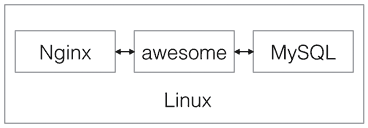
\includegraphics[width=0.6\linewidth]{fig/1019633050057984l.png}
\end{figure}


Nginx 负责分发请求:

 
 \begin{figure}[htp]
	\centering
	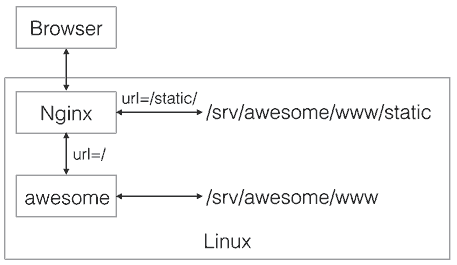
\includegraphics[width=0.6\linewidth]{fig/1019633079028160l.png}
\end{figure}


在服务器端,我们需要定义好部署的目录结构:

\begin{pythoncode}
/
+- srv/
   +- awesome/       <-- Web App根目录
      +- www/        <-- 存放Python源码
      |  +- static/  <-- 存放静态资源文件
      +- log/        <-- 存放log
\end{pythoncode}

在服务器上部署,要考虑到新版本如果运行不正常,需要回退到旧版本时怎么办。每次用新的代码覆盖掉旧的文件是不行的,需要一个类似版本控制的机制。由于
Linux
系统提供了软链接功能,所以,我们把\texttt{www}作为一个软链接,它指向哪个目录,哪个目录就是当前运行的版本:

 
 \begin{figure}[htp]
	\centering
	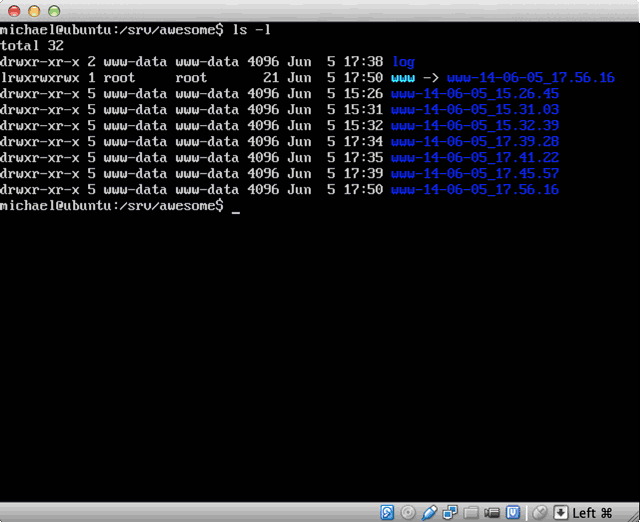
\includegraphics[width=0.6\linewidth]{fig/956187757507296.png}
\end{figure}


而 Nginx 和 python 代码的配置文件只需要指向\texttt{www}目录即可。

Nginx
可以作为服务进程直接启动,但\texttt{app.py}还不行,所以,\href{http://supervisord.org/}{Supervisor}
登场!Supervisor
是一个管理进程的工具,可以随系统启动而启动服务,它还时刻监控服务进程,如果服务进程意外退出,Supervisor
可以自动重启服务。

总结一下我们需要用到的服务有:

\begin{itemize}
\item
  Nginx:高性能 Web 服务器 + 负责反向代理;
\item
  Supervisor:监控服务进程的工具;
\item
  MySQL:数据库服务。
\end{itemize}

在 Linux 服务器上用 apt 可以直接安装上述服务:

\begin{pythoncode}
$ sudo apt-get install nginx supervisor python3 mysql-server
\end{pythoncode}

然后,再把我们自己的 Web App 用到的 Python 库安装了:

\begin{pythoncode}
$ sudo pip3 install jinja2 aiomysql aiohttp
\end{pythoncode}

在服务器上创建目录\texttt{/srv/awesome/}以及相应的子目录。

在服务器上初始化 MySQL
数据库,把数据库初始化脚本\texttt{schema.sql}复制到服务器上执行:

\begin{pythoncode}
$ mysql -u root -p < schema.sql
\end{pythoncode}

服务器端准备就绪。

\hypertarget{ux90e8ux7f72}{%
\subsubsection{部署}\label{ux90e8ux7f72}}

用 FTP 还是 SCP 还是 rsync
复制文件?如果你需要手动复制,用一次两次还行,一天如果部署 50
次不但慢、效率低,而且容易出错。

正确的部署方式是使用工具配合脚本完成自动化部署。\href{http://www.fabfile.org/}{Fabric}
就是一个自动化部署工具。由于 Fabric 是用 Python 2.x
开发的,所以,部署脚本要用 Python 2.7 来编写,本机还必须安装 Python 2.7
版本。

要用 Fabric 部署,需要在本机(是开发机器,不是 Linux 服务器)安装
Fabric:

\begin{pythoncode}
$ easy_install fabric
\end{pythoncode}

Linux 服务器上不需要安装 Fabric,Fabric 使用 SSH
直接登录服务器并执行部署命令。

下一步是编写部署脚本。Fabric
的部署脚本叫\texttt{fabfile.py},我们把它放到\texttt{awesome-python-webapp}的目录下,与\texttt{www}目录平级:

\begin{pythoncode}
awesome-python-webapp/
+- fabfile.py
+- www/
+- ...
\end{pythoncode}

Fabric 的脚本编写很简单,首先导入 Fabric 的 API,设置部署时的变量:

\begin{pythoncode}
import os, re
from datetime import datetime
from fabric.api import *
env.user = 'michael'

env.sudo_user = 'root'

env.hosts = ['192.168.0.3']
db_user = 'www-data'
db_password = 'www-data'
\end{pythoncode}

然后,每个 Python 函数都是一个任务。我们先编写一个打包的任务:

\begin{pythoncode}
_TAR_FILE = 'dist-awesome.tar.gz'

def build():
    includes = ['static', 'templates', 'transwarp', 'favicon.ico', '*.py']
    excludes = ['test', '.*', '*.pyc', '*.pyo']
    local('rm -f dist/%s' % _TAR_FILE)
    with lcd(os.path.join(os.path.abspath('.'), 'www')):
        cmd = ['tar', '--dereference', '-czvf', '../dist/%s' % _TAR_FILE]
        cmd.extend(['--exclude=\'%s\'' % ex for ex in excludes])
        cmd.extend(includes)
        local(' '.join(cmd))
\end{pythoncode}

Fabric
提供\texttt{local(\textquotesingle{}...\textquotesingle{})}来运行本地命令,\texttt{with\ lcd(path)}可以把当前命令的目录设定为\texttt{lcd()}指定的目录,注意
Fabric 只能运行命令行命令,Windows 下可能需要
\href{http://cygwin.com/}{Cgywin} 环境。

在\texttt{awesome-python-webapp}目录下运行:

\begin{pythoncode}
$ fab build
\end{pythoncode}

看看是否在\texttt{dist}目录下创建了\texttt{dist-awesome.tar.gz}的文件。

打包后,我们就可以继续编写\texttt{deploy}任务,把打包文件上传至服务器,解压,重置\texttt{www}软链接,重启相关服务:

\begin{pythoncode}
_REMOTE_TMP_TAR = '/tmp/%s' % _TAR_FILE
_REMOTE_BASE_DIR = '/srv/awesome'

def deploy():
    newdir = 'www-%s' % datetime.now().strftime('%y-%m-%d_%H.%M.%S')
    
    run('rm -f %s' % _REMOTE_TMP_TAR)
    
    put('dist/%s' % _TAR_FILE, _REMOTE_TMP_TAR)
    
    with cd(_REMOTE_BASE_DIR):
        sudo('mkdir %s' % newdir)
    
    with cd('%s/%s' % (_REMOTE_BASE_DIR, newdir)):
        sudo('tar -xzvf %s' % _REMOTE_TMP_TAR)
    
    with cd(_REMOTE_BASE_DIR):
        sudo('rm -f www')
        sudo('ln -s %s www' % newdir)
        sudo('chown www-data:www-data www')
        sudo('chown -R www-data:www-data %s' % newdir)
    
    with settings(warn_only=True):
        sudo('supervisorctl stop awesome')
        sudo('supervisorctl start awesome')
        sudo('/etc/init.d/nginx reload')
\end{pythoncode}

注意\texttt{run()}函数执行的命令是在服务器上运行,\texttt{with\ cd(path)}和\texttt{with\ lcd(path)}类似,把当前目录在服务器端设置为\texttt{cd()}指定的目录。如果一个命令需要
sudo 权限,就不能用\texttt{run()},而是用\texttt{sudo()}来执行。

\hypertarget{ux914dux7f6e-supervisor}{%
\subsubsection{配置 Supervisor}\label{ux914dux7f6e-supervisor}}

上面让 Supervisor 重启 awesome 的命令会失败,因为我们还没有配置
Supervisor 呢。

编写一个 Supervisor
的配置文件\texttt{awesome.conf},存放到\texttt{/etc/supervisor/conf.d/}目录下:

\begin{pythoncode}
[program:awesome]

command     = /srv/awesome/www/app.py
directory   = /srv/awesome/www
user        = www-data
startsecs   = 3

redirect_stderr         = true
stdout_logfile_maxbytes = 50MB
stdout_logfile_backups  = 10
stdout_logfile          = /srv/awesome/log/app.log
\end{pythoncode}

配置文件通过\texttt{{[}program:awesome{]}}指定服务名为\texttt{awesome},\texttt{command}指定启动\texttt{app.py}。

然后重启 Supervisor 后,就可以随时启动和停止 Supervisor 管理的服务了:

\begin{pythoncode}
$ sudo supervisorctl reload
$ sudo supervisorctl start awesome
$ sudo supervisorctl status
awesome                RUNNING    pid 1401, uptime 5:01:34
\end{pythoncode}

\hypertarget{ux914dux7f6e-nginx}{%
\subsubsection{配置 Nginx}\label{ux914dux7f6e-nginx}}

Supervisor 只负责运行\texttt{app.py},我们还需要配置
Nginx。把配置文件\texttt{awesome}放到\texttt{/etc/nginx/sites-available/}目录下:

\begin{pythoncode}
server {
    listen      80; 

    root       /srv/awesome/www;
    access_log /srv/awesome/log/access_log;
    error_log  /srv/awesome/log/error_log;

    

    
    location /favicon.ico {
        root /srv/awesome/www;
    }

    
    location ~ ^\/static\/.*$ {
        root /srv/awesome/www;
    }

    
    location / {
        proxy_pass       http:
        proxy_set_header X-Real-IP $remote_addr;
        proxy_set_header Host $host;
        proxy_set_header X-Forwarded-For $proxy_add_x_forwarded_for;
    }
}
\end{pythoncode}

然后在\texttt{/etc/nginx/sites-enabled/}目录下创建软链接:

\begin{pythoncode}
$ pwd
/etc/nginx/sites-enabled
$ sudo ln -s /etc/nginx/sites-available/awesome .
\end{pythoncode}

让 Nginx
重新加载配置文件,不出意外,我们的\texttt{awesome-python3-webapp}应该正常运行:

\begin{pythoncode}
$ sudo /etc/init.d/nginx reload
\end{pythoncode}

如果有任何错误,都可以在\texttt{/srv/awesome/log}下查找 Nginx 和 App
本身的 log。如果 Supervisor
启动时报错,可以在\texttt{/var/log/supervisor}下查看 Supervisor 的 log。

如果一切顺利,你可以在浏览器中访问 Linux
服务器上的\texttt{awesome-python3-webapp}了:

 
 \begin{figure}[htp]
	\centering
	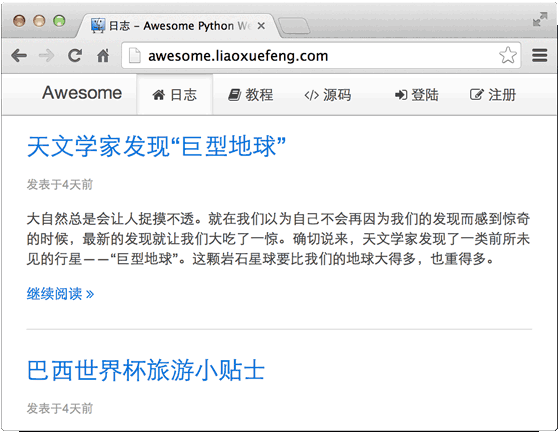
\includegraphics[width=0.6\linewidth]{fig/956196693474432.png}
\end{figure}


如果在开发环境更新了代码,只需要在命令行执行:

\begin{pythoncode}
$ fab build
$ fab deploy
\end{pythoncode}

自动部署完成!刷新浏览器就可以看到服务器代码更新后的效果。

\hypertarget{ux53cbux60c5ux94feux63a5}{%
\subsubsection{友情链接}\label{ux53cbux60c5ux94feux63a5}}

嫌国外网速慢的童鞋请移步网易和搜狐的镜像站点:

\url{http://mirrors.163.com/}

\url{http://mirrors.sohu.com/}

\hypertarget{ux53c2ux8003ux6e90ux7801}{%
\subsubsection{参考源码}\label{ux53c2ux8003ux6e90ux7801}}

\href{https://github.com/michaelliao/awesome-python3-webapp/tree/day-15}{day-15}

